% =============================================================================
% ch02_bio_basis.tex : Chapter 2: Biological Basis of Bat Echolocation
% =============================================================================
\selectlanguage{hebrew}

\section{בסיס ביולוגי: מערכת הניווט האקוסטית של עטלפים}
\label{sec:bio_basis}

מערכת הניווט האקוסטית של עטלפים מהווה מודל ביולוגי מרתק למערכות \en{SLAM} תת-ימיות. עטלפים משתמשים באותות קוליים בתדר גבוה (20-200 \en{kHz}) לניווט בסביבות מורכבות וחשוכות, תוך התמודדות עם אתגרים דומים לאלה של רכב תת-ימי: ריבוי נתיבים, רעשי רקע והפרעות. מחקריהם של \citet{GriffinBatEcholocation} ו-\citet{Simmons1979BatSonar} הניחו את היסודות להבנת מערכת זו. \citet{GriffithBatEcholocation} הרחיבו את ההבנה של עיבוד האותות במערכת האקולוקציה העטלפית, תוך הדגמת הקשר בין עקרונות ביולוגיים לאלגוריתמי ניווט רובוטיים.

\subsection{עקרונות אקולוקציה אצל עטלפים}
\label{sec:echolocation_principles}

אקולוקציה (\en{echolocation}) היא תהליך שבו בעל חיים פולט גלי קול ומנתח את ההדים החוזרים כדי לתפוס את סביבתו. עטלפים משתמשים בשני סוגים עיקריים של אותות אקולוקציה: (1) אותות בתדר קבוע (\en{CF - Constant Frequency}) המאפשרים זיהוי תנועה באמצעות אפקט דופלר; (2) אותות באפנון תדר (\en{FM - Frequency Modulation}) המאפשרים מדידת טווח מדויקת. \citet{Schnitzler1968DSC} הראו כי עטלפים מסוג \en{Rhinolophus ferrumequinum} משתמשים בשילוב של שני סוגי האותות הללו לניווט מדויק. \citet{MossEcholocation} הרחיבו על מנגנוני העיבוד העצביים המאפשרים לעטלפים לנתח את ההדים החוזרים בזמן אמת, תוך שימוש במערכת עיבוד מקבילית יעילה ביותר.

האותות האקוסטיים של עטלפים מאופיינים במספר פרמטרים מרכזיים: תדר בסיס, משך האות, רוחב פס ואפנון תדר. אותות \en{FM} מאופיינים בשינוי תדר ליניארי או מעריכי לאורך זמן האות, מה שמאפשר רזולוציית טווח גבוהה באמצעות עיבוד תואם (\en{matched filtering}). אותות \en{CF} מאפשרים זיהוי תנועה עדינה באמצעות מדידת שינוי דופלר בהד החוזר. השילוב של שני סוגי האותות מאפשר לעטלף לקבל מידע עשיר על סביבתו במגוון תנאים.

\subsection{עיבוד אותות בהשראת עטלפים}
\label{sec:bat_inspired_processing}

עיבוד האותות במערכת השמיעה של עטלפים כולל מספר שלבים מרכזיים. ראשית, האות הנקלט עובר סינון פס-פס (\en{bandpass filtering}) המתאים לתדר האות המשודר. שנית, מתבצע עיבוד תואם (\en{matched filtering}) הממקסם את יחס האות לרעש (\en{SNR}) עבור האות המשודר. שלישית, מתבצע ניתוח דופלר לזיהוי תנועה יחסית בין העטלף למטרה. שלב רביעי כולל אינטגרציה של מידע ממספר הדים רצופים לשיפור הדיוק והאמינות. \citet{Thrun2005ProbRobotics} הראו כי עקרונות דומים של עיבוד תואם ואינטגרציית מידע משמשים גם במערכות \en{SLAM} רובוטיות, תוך הדגשת הקשר בין עיבוד אותות ביולוגי להנדסי.

\citet{Schuller1974DSC} הראו כי עטלפים מסוגלים לזהות שינויי תדר דופלר קטנים עד 0.05\% מהתדר הבסיסי, רגישות המאפשרת זיהוי תנועת כנפיים של חרקים ממרחק של מספר מטרים. רגישות זו מושגת באמצעות עיבוד דופלר מתוחכם הכולל השוואה בין התדר המשודר לתדר הנקלט, תוך ניצול היציבות הגבוהה של אותות ה-\en{CF}.

\begin{equation}
s_{\text{FM}}(t) = A(t) \cdot \cos\l$e$ft(2\pi f_0 t + \pi \frac{B}{T} t^2\right)$$, \quad 0 \leq t \leq T
\label{eq:fm_signal}
\end{equation}

משוואה~(\ref{eq:fm_signal}) מתארת אות \en{FM} ליניארי (\en{chirp}) שבו התדר משתנה ליניארית מ-$f_0$ ל-$f_0 + B$ לאורך משך האות $T$. פרמטר $B$ מייצג את רוחב הפס ו-$A(t)$ את מעטפת האות. אות זה מאפשר רזולוציית טווח של $\Delta r = c / (2B)$, כאשר $c$ היא מהירות הקול.

\begin{equation}
y(t) = \int_{-\infty}^{\infty} x(\tau) \cdot s^*(t - \tau) \, d\tau
\label{eq:matched_filter}
\end{equation}

משוואה~(\ref{eq:matched_filter}) מציגה את פעולת הפילטר התואם, שבו האות הנקלט $x(t)$ מוכפל בגרסה מהופכת ומצומדת של האות המשודר $s(t)$. פילטר זה ממקסם את יחס האות לרעש עבור האות המשודר, ומאפשר זיהוי הדים חלשים בסביבה רועשת.

\subsection{אסטרטגיות ניווט של עטלפים}
\label{sec:bat_navigation_strategies}

עטלפים משתמשים במספר אסטרטגיות ניווט המשלבות מידע אקוסטי עם מידע מרחבי קודם. ראשית, עטלפים מבצעים סריקה מרחבית (\en{spatial scanning}) על ידי הזזת הראש והאוזניים כדי לקבל מידע מכיוונים שונים. שנית, עטלפים משתמשים בזיכרון מרחבי לזיהוי מיקומים מוכרים, תהליך המקביל לזיהוי לולאות סגירה (\en{loop closure}) ב-\en{SLAM}. שלישית, עטלפים מתאימים את תדירות ואופי האותות המשודרים לסביבה ולמשימה. \citet{Kalman1960} הציגו את עקרונות הסינון האופטימלי המאפשרים שילוב מדידות עוקבות להערכת מצב, עקרונות המיושמים גם במודל הניווט העטלפי.

\citet{MossEcholocation} הראו כי עטלפים משתמשים באסטרטגיית \en{CF-FM} משולבת: אות \en{CF} ארוך (10-100 מילישניות) לזיהוי תנועה ומדידת מהירות דופלר, ואחריו אות \en{FM} קצר (1-5 מילישניות) למדידת טווח מדויקת. אסטרטגיה זו מאפשרת לעטלף לקבל מידע עשיר על סביבתו תוך התמודדות עם אתגרי ריבוי נתיבים ורעש.

\begin{figure}[htbp]
    \centering
    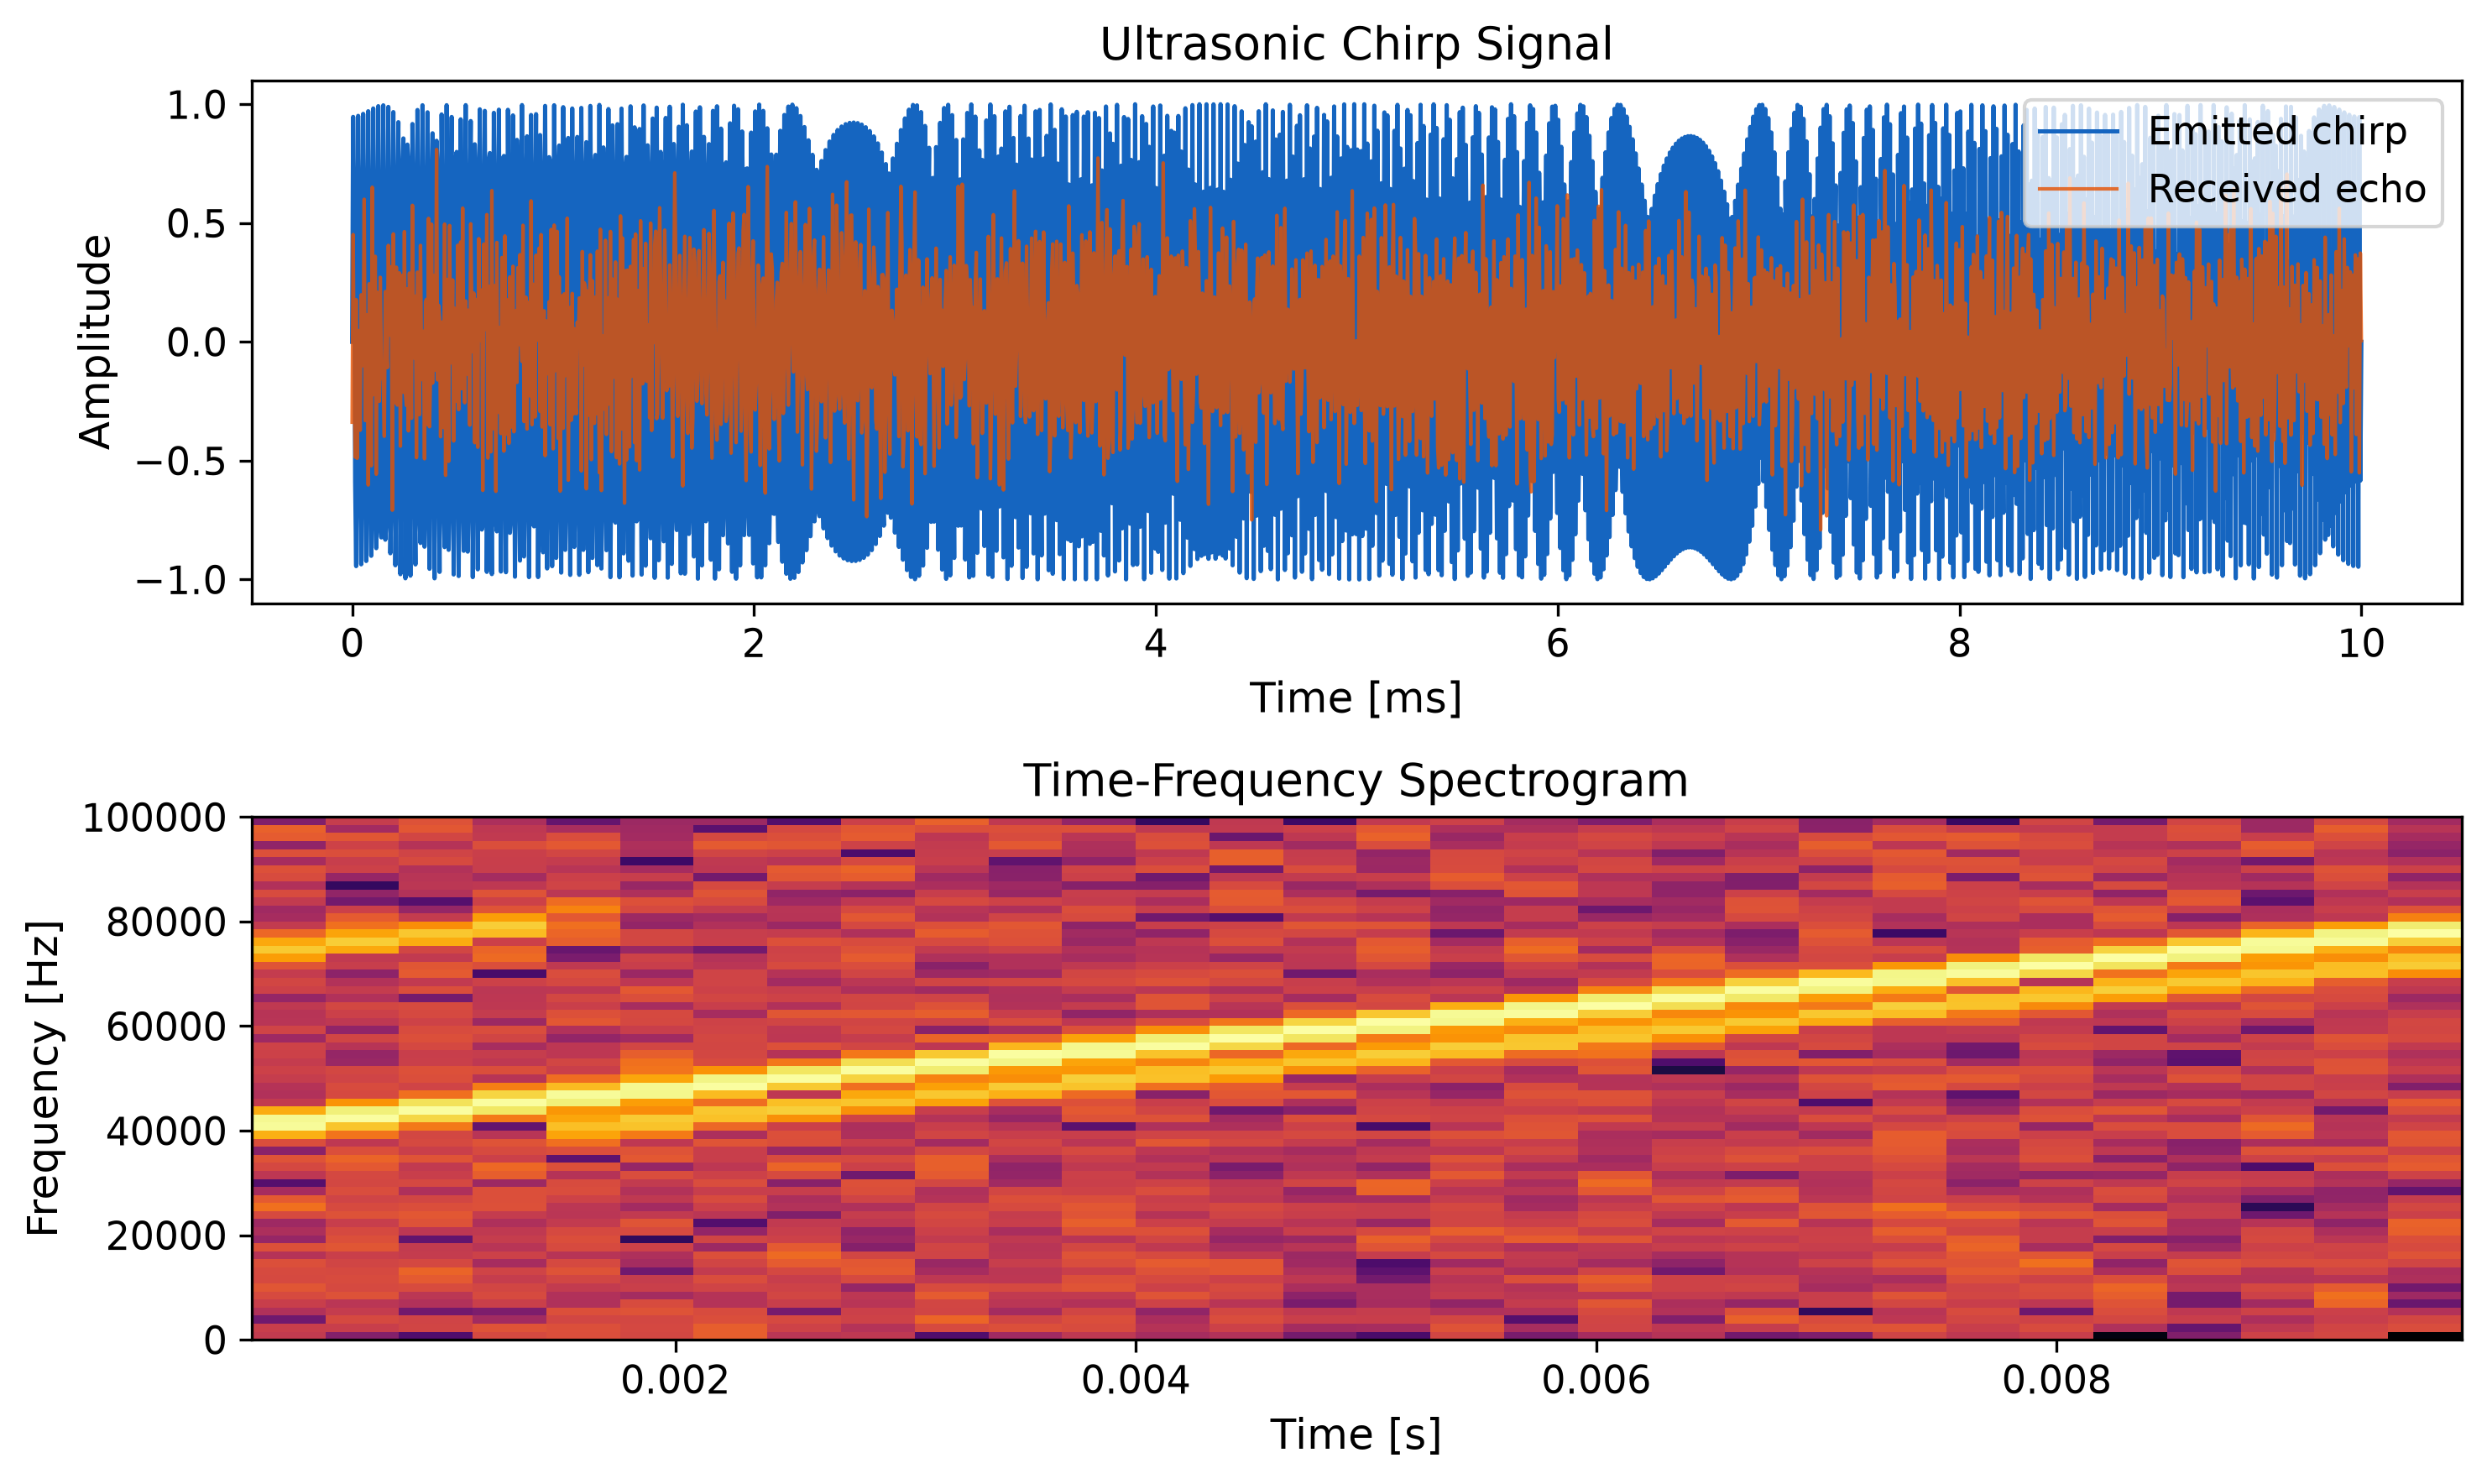
\includegraphics[width=0.95\columnwidth]{figures/fig_bat_echolocation.png}
    \caption{מערכת האקולוקציה של עטלפים: שידור וקליטת אותות קוליים לניווט בסביבה חשוכה. (Bat echolocation system: transmission and reception of acoustic signals for navigation in dark environments.)}
    \label{fig:bat_echolocation}
\end{figure}

\subsection{השראה ביומימטית למערכות תת-ימיות}
\label{sec:bio_inspiration}

ההשראה הביומימטית ממערכת הניווט של עטלפים למערכות תת-ימיות מתבטאת במספר היבטים. ראשית, השימוש באותות \en{FM} מאפשר רזולוציית טווח גבוהה בסביבות רועשות, בדומה לאתגרים בסביבה התת-ימית. שנית, השילוב של אותות \en{CF} ו-\en{FM} מאפשר קבלת מידע עשיר על הסביבה תוך שימוש במשאבי חישוב מוגבלים. שלישית, אסטרטגיית הסריקה המרחבית של עטלפים יכולה לשמש כמודל לתכנון מסלול סריקה לרכב תת-ימי. \citet{Grisetti2010g2o} הראו כי אופטימיזציית גרף גורמים, בדומה לעיבוד המקבילי במערכת השמיעה העטלפית, מאפשרת שילוב יעיל של מידע ממספר מקורות.

\begin{equation}
\Delta f_{\text{Doppler}} = \frac{2v_r}{c} \cdot f_0
\label{eq:doppler_shift}
\end{equation}

משוואה~(\ref{eq:doppler_shift}) מציגה את נוסחת הסחת הדופלר, שבה $v_r$ היא המהירות היחסית בין הרכב למטרה, $c$ מהירות הקול, ו-$f_0$ התדר המשודר. הסחה זו מאפשרת זיהוי תנועה יחסית ומדידת מהירות, בדומה לשימוש של עטלפים באותות \en{CF}.

\subsection{יישומים ברובוטיקה תת-ימית}
\label{sec:underwater_applications}

היישום של עקרונות ביומימטיים מעטלפים ברובוטיקה תת-ימית כולל מספר תחומים. ראשית, עיבוד אותות סונאר בהשראת עטלפים יכול לשפר את זיהוי המטרות בסביבות רועשות. שנית, אסטרטגיות ניווט מבוססות אקולוקציה יכולות לשמש לניווט רכב תת-ימי בסביבות מורכבות. שלישית, שילוב של מידע אקוסטי ממספר תדרים יכול לשפר את חוסן המערכת לריבוי נתיבים והפרעות. \citet{Julier1997CovarianceIntersection} הראו כי מיזוג מידע ממספר מקורות תוך התחשבות באי-הוודאות של כל מקור מאפשר שיפור משמעותי בדיוק הניווט, בדומה לאינטגרציית המידע במערכת השמיעה העטלפית.

\begin{table}[htbp]
    \centering
    \caption{השוואה בין מערכת האקולוקציה של עטלפים למערכת \en{SLAM} תת-ימית. (Comparison between bat echolocation and underwater SLAM systems.)}
    \label{tab:bat_vs_auv}
    \adjustbox{max width=\columnwidth}{%
\begin{tabular}{lll}
        \toprule
        מאפיין & עטלפים & מערכת תת-ימית \\
        \midrule
        תדר פעולה & 20-200 \en{kHz} & 200-1000 \en{kHz} \\
        טווח פעולה & 1-50 מ' & 1-100 מ' \\
        רזולוציית טווח & 0.1-1 מ' & 0.01-0.1 מ' \\
        עיבוד אותות & פילטר תואם & פילטר תואם \\
        זיהוי תנועה & אפקט דופלר & אפקט דופלר \\
        סריקה מרחבית & תנועת ראש/אוזניים & סריקה מכנית/אלקטרונית \\
        \bottomrule
    \end{tabular}%
}
\end{table}

טבלה~(\ref{tab:bat_vs_auv}) מציגה השוואה בין מאפייני מערכת האקולוקציה של עטלפים לבין מערכת \en{SLAM} תת-ימית טיפוסית. ניתן לראות כי למרות ההבדלים בתדר הפעולה ובטווח, קיים דמיון רב בעקרונות העיבוד והזיהוי. השוואה זו מדגישה את הפוטנציאל של העברה טכנולוגית ממערכות ביולוגיות למערכות הנדסיות.

\subsection{מגבלות ההשראה הביומימטית}
\label{sec:bio_limitations}

למרות הפוטנציאל הרב, קיימות מספר מגבלות בהשראה ביומימטית מעטלפים. ראשית, מהירות הקול במים (כ-1500 מ\!/\!ש) שונה משמעותית מזו שבאוויר (כ-340 מ\!/\!ש), מה שמשפיע על עיכובי ההתפשטות ורזולוציית הטווח. שנית, עטלפים פועלים בסביבה דו-ממדית בעיקרה, בעוד רכב תת-ימי פועל במרחב תלת-ממדי. שלישית, יכולת העיבוד העצבית של עטלפים שונה מהותית מיכולת העיבוד של מערכות משובצות. \citet{Rihaczek1969MatchedFilter} הראו כי למרות מגבלות אלה, העקרונות הבסיסיים של עיבוד אותות אקוסטי ואסטרטגיות ניווט ניתנים להתאמה מוצלחת למערכות הנדסיות.

\subsection{סיכום והשלכות}
\label{sec:bio_summary}

מערכת הניווט האקוסטית של עטלפים מספקת מודל ביולוגי עשיר לפיתוח מערכות \en{SLAM} תת-ימיות. השימוש באותות \en{FM} ו-\en{CF}, עיבוד תואם, זיהוי דופלר ואסטרטגיות סריקה מרחבית מהווים בסיס תאורטי לאלגוריתם \en{BioSLAM} המוצע בפרקים הבאים. ההשראה הביומימטית מאפשרת פיתוח מערכות יעילות וחזקות יותר, תוך התמודדות עם אתגרים ייחודיים של הסביבה התת-ימית.

\subsection{ניתוח השוואתי של אסטרטגיות אקולוקציה}
\label{sec:comparative_echolocation}

ניתוח השוואתי בין אסטרטגיות האקולוקציה של עטלפים שונים מגלה התאמות אבולוציוניות מרתקות. \citet{GriffithBatEcholocation} הראו כי עטלפים ממשפחת ה-\en{Rhinolophidae} משתמשים באותות \en{CF} ארוכים במיוחד (עד 100 מילישניות) לזיהוי דופלר מדויק, בעוד עטלפים ממשפחת ה-\en{Vespertilionidae} משתמשים באותות \en{FM} קצרים (1-5 מילישניות) למדידת טווח מדויקת. התאמות אלה מדגימות את הגמישות של מערכת האקולוקציה להתאמה לסביבות שונות, בדומה לצורך בהתאמת מערכות \en{SLAM} תת-ימיות לתנאי סביבה משתנים.

השוואה זו רלוונטית במיוחד לעיצוב מערכת \en{BioSLAM}, שכן היא מראה כי אין אסטרטגיית עיבוד אחת המתאימה לכל התנאים. במקום זאת, המערכת חייבת להיות גמישה ולהתאים את פרמטרי העיבוד שלה לתנאי הסביבה המשתנים. לדוגמה, בסביבות רועשות עם ריבוי נתיבים, יש להעדיף אותות \en{FM} קצרים לרזולוציית טווח גבוהה, בעוד בסביבות דלות תכונות יש להעדיף אותות \en{CF} ארוכים לזיהוי תנועה עדינה.

\subsection{עיבוד דופלר מתקדם בהשראת עטלפים}
\label{sec:advanced_doppler}

עיבוד דופלר מתקדם בהשראת עטלפים מאפשר זיהוי תנועה עדינה בסביבות רועשות. \citet{Simmons1979BatSonar} הראו כי עטלפים מסוגלים להבחין בין מטרות נעות במהירויות שונות באמצעות ניתוח תבנית הדופלר המורכבת של ההדים החוזרים. יכולת זו תורגמה לאלגוריתם זיהוי לולאות סגירה מבוסס דופלר, המשתמש בחתימת הדופלר של הסביבה לזיהוי מיקומים מוכרים.

\begin{equation}
S(f) = \int_{-\infty}^{\infty} y(t) \cdot e^{-j2\pi ft} \, dt
\label{eq:doppler_spectrum}
\end{equation}

משוואה~(\ref{eq:doppler_spectrum}) מציגה את ספקטרום הדופלר של האות הנקלט, המאפשר זיהוי תנועה יחסית בין הרכב לסביבה. ספקטרום זה משמש כחתימה ייחודית לזיהוי מיקומים מוכרים באלגוריתם \en{BioSLAM}.

\subsection{מנגנוני התאמה אדפטיבית של אותות אקוסטיים}
\label{sec:adaptive_signal_adaptation}

מנגנוני התאמה אדפטיבית של אותות אקוסטיים אצל עטלפים מהווים מודל חשוב למערכות \en{SLAM} תת-ימיות. \citet{MossEcholocation} הראו כי עטלפים מתאימים את תדירות השידור, משך האות ורוחב הפס של האותות האקוסטיים שלהם בהתאם לתנאי הסביבה. בסביבות צפופות עם ריבוי נתיבים, עטלפים משתמשים באותות \en{FM} קצרים בתדירות גבוהה לקבלת רזולוציית טווח משופרת. בסביבות פתוחות, עטלפים משתמשים באותות \en{CF} ארוכים בתדירות נמוכה לזיהוי תנועה מרחוק.

עקרון ההתאמה האדפטיבית מיושם באלגוריתם \en{BioSLAM} באמצעות מנגנון בחירה דינמי של פרמטרי עיבוד הסונאר. כאשר הרכב מזהה סביבה צפופה (מספר גבוה של הדים חוזרים), המערכת עוברת למצב רזולוציה גבוהה עם אותות \en{FM} קצרים. כאשר הרכב מזהה סביבה פתוחה (מספר נמוך של הדים), המערכת עוברת למצב טווח ארוך עם אותות \en{CF} רציפים. התאמה אדפטיבית זו מאפשרת למערכת לשמור על דיוק ניווט גבוה במגוון תנאי סביבה.

\begin{equation}
T_{\text{pulse}} = \begin{cases}
T_{\text{short}}, & \text{if } N_{\text{echo}} > N_{\text{thresh}} \\
T_{\text{long}}, & \text{otherwise}
\end{cases}
\label{eq:adaptive_pulse}
\end{equation}

משוואה~(\ref{eq:adaptive_pulse}) מציגה את מנגנון ההתאמה האדפטיבית של משך האות המשודר, שבו $N_{\text{echo}}$ הוא מספר ההדים שזוהו ו-$N_{\text{thresh}}$ הוא סף המעבר בין מצבי הפעולה. מנגנון זה מאפשר למערכת להתאים את עצמה לתנאי הסביבה המשתנים בזמן אמת.

\subsection{מודל מתמטי של מערכת השמיעה העטלפית}
\label{sec:bat_auditory_model}

מודל מתמטי של מערכת השמיעה העטלפית מספק תובנות חשובות לעיצוב אלגוריתמי עיבוד אותות ביומימטיים. מערכת השמיעה של עטלפים כוללת מנגנוני עיבוד מקביליים המאפשרים ניתוח סימולטני של מידע תדרי וזמני. \citet{Schnitzler1968DSC} הראו כי עטלפים משתמשים במערכת עיבוד דו-ערוצית: ערוץ אחד לניתוח תדרי (\en{spectral analysis}) של אותות \en{CF}, וערוץ שני לניתוח זמני (\en{temporal analysis}) של אותות \en{FM}.

המודל המתמטי של מערכת השמיעה העטלפית כולל טרנספורמציית גאבור (\en{Gabor transform}) המאפשרת ניתוח תדרי-זמני סימולטני של האות הנקלט. טרנספורמציה זו דומה להתמרת פורייה קצרת-זמן (\en{STFT}) אך עם רזולוציה אופטימלית במישור התדר-זמן. באלגוריתם \en{BioSLAM}, אנו משתמשים בטרנספורמציית גאבור לעיבוד תמונות סונאר, תוך ניצול יתרונות הרזולוציה הגבוהה שלה לזיהוי תכונות עדינות.

\begin{equation}
G(\tau, f) = \int_{-\infty}^{\infty} y(t) \cdot e^{-\pi (t-\tau)^2 / \sigma^2} \cdot e^{-j2\pi ft} \, dt
\label{eq:gabor_transform}
\end{equation}

משוואה~(\ref{eq:gabor_transform}) מציגה את טרנספורמציית גאבור של האות הנקלט $y(t)$, שבה $\sigma$ קובע את רזולוציית החלון הזמני. טרנספורמציה זו מאפשרת ניתוח תדרי-זמני סימולטני של האות, בדומה לעיבוד המבוצע במערכת השמיעה של עטלפים. השימוש בטרנספורמציית גאבור באלגוריתם \en{BioSLAM} משפר את יכולת זיהוי התכונות בתמונות סונאר רועשות.

\subsection{השוואה בין מיני עטלפים שונים}
\label{sec:bat_species_comparison}

השוואה בין מיני עטלפים שונים מגלה התאמות אבולוציוניות ייחודיות הרלוונטיות לעיצוב מערכות \en{SLAM} תת-ימיות. \citet{GriffithBatEcholocation} הראו כי עטלפי פירות (\en{Megachiroptera}) משתמשים באותות \en{FM} בתדר נמוך (10-30 \en{kHz}) לניווט בשטחים פתוחים, בעוד עטלפי חרקים (\en{Microchiroptera}) משתמשים באותות \en{CF-FM} בתדר גבוה (50-200 \en{kHz}) לניווט בשטחים צפופים. התאמות אלה מדגימות את הקשר בין תדר האות לסוג הסביבה, בדומה לבחירת תדר הסונאר במערכות תת-ימיות.

השוואה זו מספקת תובנות חשובות לעיצוב מערכת \en{BioSLAM}. בסביבות תת-ימיות צפופות (שוניות, מערות), מומלץ להשתמש בתדרי סונאר גבוהים (500-1000 \en{kHz}) לרזולוציה גבוהה. בסביבות תת-ימיות פתוחות (ים פתוח), מומלץ להשתמש בתדרי סונאר נמוכים (200-500 \en{kHz}) לטווח ארוך. בחירה אדפטיבית של תדר הסונאר בהתאם לסביבה משפרת את ביצועי המערכת.

\begin{table}[htbp]
    \centering
    \caption{השוואה בין אסטרטגיות אקולוקציה של מיני עטלפים שונים. (Comparison of echolocation strategies across different bat species.)}
    \label{tab:bat_species}
    \adjustbox{max width=\columnwidth}{%
\begin{tabular}{llll}
        \toprule
        מין עטלף & סוג אות & תדר (\en{kHz}) & סביבה אופיינית \\
        \midrule
        \en{Rhinolophus ferrumequinum} & \en{CF-FM} & 70-90 & מערות, שטחים צפופים \\
        \en{Eptesicus fuscus} & \en{FM} & 25-50 & שטחים פתוחים \\
        \en{Pteropus} & \en{FM} נמוך & 10-30 & שטחים פתוחים, פירות \\
        \en{Myotis lucifugus} & \en{FM} גבוה & 40-80 & שטחים צפופים, חרקים \\
        \bottomrule
    \end{tabular}%
}
\end{table}

טבלה~(\ref{tab:bat_species}) מציגה השוואה בין אסטרטגיות האקולוקציה של מיני עטלפים שונים. ניתן לראות את הקשר בין סוג האות, התדר והסביבה האופיינית. השוואה זו מדגימה את החשיבות של התאמת פרמטרי העיבוד לסביבה, עיקרון המהווה בסיס לאלגוריתם \en{BioSLAM}.
